\documentclass[11pt,a4paper]{article}
\usepackage[margin=1in]{geometry}
\usepackage{amsmath,amssymb,amsthm}
\usepackage{algorithm}
\usepackage{algpseudocode}
\usepackage{booktabs}
\usepackage{enumitem}
\usepackage{hyperref}
\usepackage{xcolor}
\usepackage{graphicx}

\newcommand{\bX}{\mathbf{X}}
\newcommand{\bY}{\mathbf{Y}}
\newcommand{\bbeta}{\boldsymbol{\beta}}
\newcommand{\beps}{\boldsymbol{\varepsilon}}
\newcommand{\bI}{\mathbf{I}}
\newcommand{\RE}{\mathrm{RE}}
\newcommand{\MSE}{\mathrm{MSE}}
\newcommand{\tr}{\mathrm{tr}}
\newcommand{\OLS}{\mathrm{OLS}}
\begin{document}
\section{Experimental results}
This simulation is designed to examine the effect of our proposed Distributed Global Subsampled Randomized Hadamard Transform (DGSRHT) algorithm ~\ref{alg:example} on the empirical training efficiency and theoretical relative efficiency of equal-weight distributed OLS under the heterogeneous Gaussian mixture model introduced in Definition~\ref{def:gmm}.
\subsection{Simulation design}

The simulations are designed to examine the finite-sample behavior of equal-weight distributed OLS under the heterogeneous Gaussian mixture model introduced in Definition~\ref{def:gmm}. Throughout this section we fix the total sample size at $n=32768$, the number of initial client machines in the DGSRHT pipeline at $K=16$, and the feature dimension at $p=60$. The mixture parameters are set to $a_{1}=0.8$, $\mu_{1}=0$, $\mu_{2}=5$, and covariance inflation factor $c=10$, so that the second mixture component has substantially larger dispersion. The client-side keep proportion in the sketching stage is fixed at $1/s=0.25$, hence $s=4$.

For each simulation run, we first generate a regression vector $\beta_{\ast}\in\mathbb{R}^{p}$ from $\mathcal{N}(0,\mathbf{I}_{p})$. We then generate a random positive definite covariance matrix
\[
\Sigma_{1}=\frac{AA^{\top}}{p}+10^{-3}\mathbf{I}_{p},
\]
where the entries of $A$ are i.i.d.\ standard normal, and set $\Sigma_{2}=c\Sigma_{1}$. The initial client sizes $m_{1},\ldots,m_{K}$ are drawn once from the function \texttt{multinomial\_no\_zeros}, which guarantees $m_{i}\geq 1$ and $\sum_{i=1}^{K} m_{i}=n$ while allowing heterogeneous local sample sizes. Conditional on these quantities, each row on client $i$ is drawn independently from the two-component mixture
\[
x \sim a_{1}\,\mathcal{N}_{p}(\mu_{1}\mathbf{1}_{p},\Sigma_{1}) + (1-a_{1})\,\mathcal{N}_{p}(\mu_{2}\mathbf{1}_{p},\Sigma_{2}).
\]
For the DGSRHT pipeline, each local design is padded to
\[
m_{\mathrm{loc}} = 2^{\lceil \log_{2}(\max_{1\leq i\leq K} m_{i}) \rceil}
\]
rows, exactly as in Algorithm~\ref{alg:example}. The design matrices are generated once and then held fixed throughout the Monte Carlo repetitions.

Given this fixed design, for each repetition $r=1,\ldots,R$ with $R=300$, we draw fresh observation noise independently on every client:
\[
\varepsilon_{i}^{(r)} \sim \mathcal{N}(0,\mathbf{I}_{m_{i}}), \qquad
Y_{i}^{(r)} = X_{i}\beta_{\ast} + \varepsilon_{i}^{(r)}.
\]
Hence the averaging over repetitions isolates the effect of response noise together with the randomness introduced by the partitioning and sketching steps, while keeping the underlying heterogeneous design fixed.

\subsection{Compared pipelines and evaluation protocol}

We compare two pipelines.

\paragraph{Uniform local-sampling baseline.}
On client $i$, we sample
\[
r_{i}=\max\{1,\mathrm{round}(m_{i}/s)\}
\]
rows uniformly without replacement from the raw data $(X_{i},Y_{i})$, and then stack all selected rows. This is the implementation \texttt{baseline\_uniform\_local\_rate} in the notebook. The baseline therefore matches the DGSRHT pipeline at the level of the local keep proportion $1/s$.

\paragraph{DGSRHT pipeline.}
We implement Algorithm~\ref{alg:example} exactly as written in the notebook: local shuffle, local randomized Hadamard transform, one shared row-selection operator keeping $r=m_{\mathrm{loc}}/s$ rows per client, server-side Hadamard mixing $(H_{K}\otimes I_{r})$, and the final scaling by $\sqrt{s}$. The resulting global sketched dataset is the pair $(\tilde X_{\star},\tilde Y_{\star})$ returned by \texttt{server\_mixer}.

After either pipeline produces a global sketched dataset $(Z,V)$, we study distributed OLS on top of that dataset. For each number of working machines
\[
K' \in \{1,2,\ldots,30\},
\]
we repartition the rows of $(Z,V)$ uniformly at random into $K'$ nearly equal blocks, compute the local OLS estimator on each block, and aggregate the local coefficients by the equal-weight average from Algorithm~\ref{alg:example2}. The centralized comparator is the OLS estimator computed on the full sketched dataset $(Z,V)$ itself. Consequently, the relative efficiency is equal to one when $K'=1$.

A small implementation detail is worth stating explicitly for reproducibility. The two methods are matched by the client-side keep proportion $1/s$, but not necessarily by the final total row count. The uniform baseline returns $\sum_{i=1}^{K} r_{i}$ sampled raw rows, whereas the DGSRHT pipeline returns $Kr$ rows because it operates after padding all clients to the common size $m_{\mathrm{loc}}$. This is the exact logic implemented in \texttt{new\_simulation\_1.ipynb}, and the paper reports the corresponding outputs without any post hoc row-count adjustment.

\subsection{Relative-efficiency metric}

For a realized sketched dataset $(Z^{(r)},V^{(r)})$ at repetition $r$, let $\widehat{\beta}_{\mathrm{cen}}^{(r)}$ denote the centralized OLS estimator on the full sketched data, and let $\widehat{\beta}_{\mathrm{dist},K'}^{(r)}$ denote the equal-weight distributed OLS estimator obtained after repartitioning the same sketched data into $K'$ working machines. The empirical relative efficiency reported in Figure~\ref{fig:exp_re} is
\[
\mathrm{RE}_{\mathrm{emp}}(K')
=
\frac{\frac{1}{R}\sum_{r=1}^{R}\|\widehat{\beta}_{\mathrm{cen}}^{(r)}-\beta_{\ast}\|_{2}^{2}}
{\frac{1}{R}\sum_{r=1}^{R}\|\widehat{\beta}_{\mathrm{dist},K'}^{(r)}-\beta_{\ast}\|_{2}^{2}}.
\]
Thus, the numerator and denominator are both empirical mean squared parameter-estimation errors measured against the same ground-truth vector $\beta_{\ast}$.

In addition to the empirical curves, we also plot a design-conditional finite-sample benchmark computed from the exact OLS risk identities in Lemma~\ref{lem:finiteresults} with $A=I_{p}$ and equal weights $w_{j}=1/K'$. For a realized design matrix $Z$ and a realized repartition $Z_{1},\ldots,Z_{K'}$, the benchmark is
\[
\mathrm{RE}_{\mathrm{bench}}(K';Z)
=
\frac{\operatorname{tr}\!\bigl[(Z^{\top}Z)^{-1}\bigr]}
{\sum_{j=1}^{K'} (1/K')^{2}\operatorname{tr}\!\bigl[(Z_{j}^{\top}Z_{j})^{-1}\bigr]}.
\]
In the notebook this benchmark is evaluated once using the first realized design produced by each pipeline. Accordingly, it should be read as a finite-sample plug-in benchmark for a realized design, rather than as an additional Monte Carlo average.

\subsection{Main findings}

\begin{figure}[t]
    \centering
    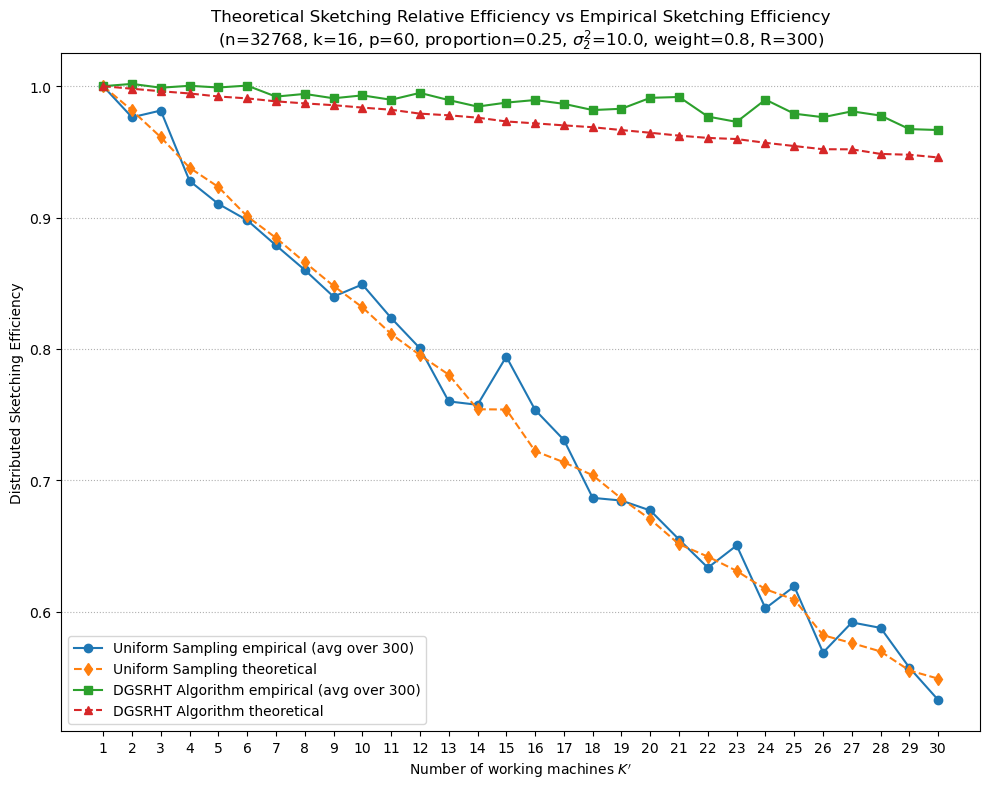
\includegraphics[width=0.92\textwidth]{result_graph.png}
    \caption{Empirical and design-conditional benchmark relative efficiency as a function of the number of working machines $K'$. The empirical curves are averaged over $R=300$ repetitions. Parameters are fixed at $n=32768$, $K=16$, $p=60$, $a_{1}=0.8$, $\mu_{1}=0$, $\mu_{2}=5$, covariance inflation factor $c=10$, and keep proportion $1/s=0.25$.}
    \label{fig:exp_re}
\end{figure}

Figure~\ref{fig:exp_re} shows a clear qualitative separation between the two pipelines. For the uniform local-sampling baseline, the empirical relative efficiency decreases steadily as $K'$ grows, dropping from $1$ at $K'=1$ to approximately $0.53$ at $K'=30$. The corresponding benchmark curve follows the same monotone pattern. This behavior indicates that, under the raw heterogeneous GMM design, equal-weight averaging becomes increasingly sensitive to block-to-block variation in the local Gram matrices as the number of working machines increases.

By contrast, the DGSRHT pipeline remains substantially more stable. Across the full range $K'=1,\ldots,30$, the empirical relative efficiency stays close to one, fluctuating only mildly around the interval $[0.97,1.00]$. The benchmark curve also decays much more slowly, remaining around $0.95$ even at $K'=30$. In practical terms, this means that after DGSRHT preprocessing, repartitioning the sketched data over many working machines causes only a small loss relative to centralized OLS on the same sketched dataset.

The comparison is consistent with the mechanism developed in the theory sections of the paper. The raw GMM design creates uneven row magnitudes and consequently uneven local Gram matrices under uniform partitioning, which makes equal-weight aggregation inefficient. The randomized Hadamard preprocessing mixes these heterogeneous rows before repartitioning, so the resulting local least-squares problems are markedly better balanced. The empirical curves therefore support the main message of Corollary~\ref{corollary:main}: DGSRHT makes equal-weight averaging much closer to the centralized benchmark, even when the number of downstream working machines is large.

Finally, the gap between the empirical DGSRHT curve and its benchmark curve should not be over-interpreted. The benchmark is computed conditionally on a single realized sketched design, whereas the empirical curve averages over 300 repetitions with fresh response noise and fresh partitioning/sketch randomness. The remaining discrepancy is therefore a finite-sample Monte Carlo effect, not a qualitative contradiction.

\section{Discussion}
The experiments support the main theoretical message of this paper. When the design matrix is generated from the heterogeneous Gaussian mixture model of Definition~\ref{def:gmm}, equal-weight distributed OLS after raw uniform sampling loses efficiency rapidly as the number of working machines increases. In contrast, the DGSRHT preprocessing substantially stabilizes the local Gram matrices and preserves near-centralized performance under the same equal-weight aggregation rule.

Our current theoretical result is still tailored to the GMM setting and to the asymptotic regime described in Remark~\ref{remark:sublinear}. Two natural directions remain open. The first is to extend the analysis to broader families of heterogeneous designs, for instance more general elliptical or heavy-tailed row distributions. The second is to study regimes in which $p$ is genuinely comparable to $n$, such as $p=c_{1}n$ for a fixed constant $c_{1}\in(0,1)$. A sharper finite-sample analysis of the gap between the design-conditional benchmark and the Monte Carlo averages in Figure~\ref{fig:exp_re} would also be of independent interest.
\end{document}